\documentclass[aspectratio=169, hyperref={colorlinks=true}]{beamer}
\usepackage[beamer, collink]{prettytex/base}
\usepackage{prettytex/math}
\usepackage{prettytex/gfx}
\usepackage{csquotes}
\usepackage[backend=biber, style=numeric, maxbibnames=20]{biblatex}
% \usepackage[acronym, style=long3col, indexonlyfirst=true, nogroupskip=true]{glossaries}
\usetheme[serif, sansserifheader]{tugrazivc}

\usefonttheme{default}
\addtobeamertemplate{frametitle}{}{\vspace*{-1em}}

% \makeglossaries
% \newacronym[shortplural=IAIs, longplural=interpretable artifical intelligence]{iai}{IAI}{interpretable artificial intelligence}


\addbibresource{../../literature/sources.bib}

\title[IVC Seminar SS2025]{In-Silico Cancer Cell}
\author[Peter Waldert]{\textbf{Peter Waldert}}
\date{\today}
\institute{IVC}
\instituteurl{ivc.tugraz.at}

\begin{document}
  \begin{frame}[plain]
    \maketitle
  \end{frame}

  \begin{frame}{Biological Setting: Cancer Cell}
    %% A549 model (lung cancer)
    %% with picture
    \begin{columns}
      \begin{column}{0.4\linewidth}
        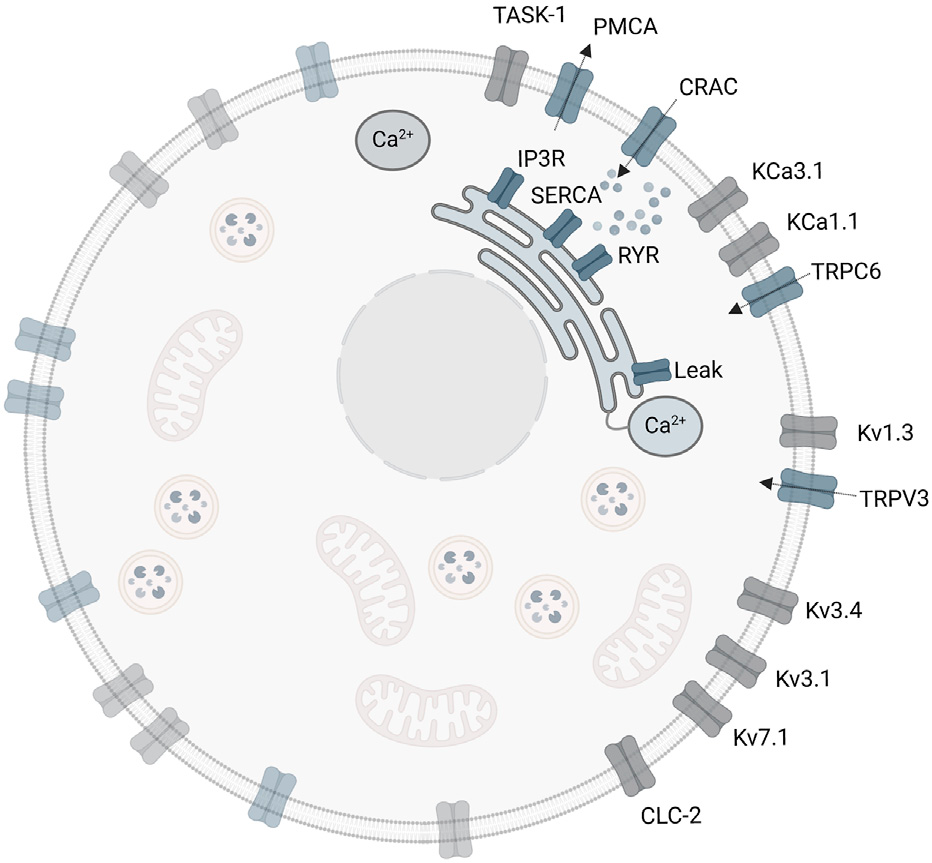
\includegraphics[width=\linewidth]{../../figures/cell-by-langthaler-et-al.png}
      \end{column}
      \begin{column}{0.58\linewidth}
        Indeed
      \end{column}
    \end{columns}
  \end{frame}

  \begin{frame}{Experiment: Patch-Clamping}
    %% describe, with picture
    %% we measure current based on voltage changes
    \begin{columns}
      \begin{column}{0.4\linewidth}
        \begin{figure}
          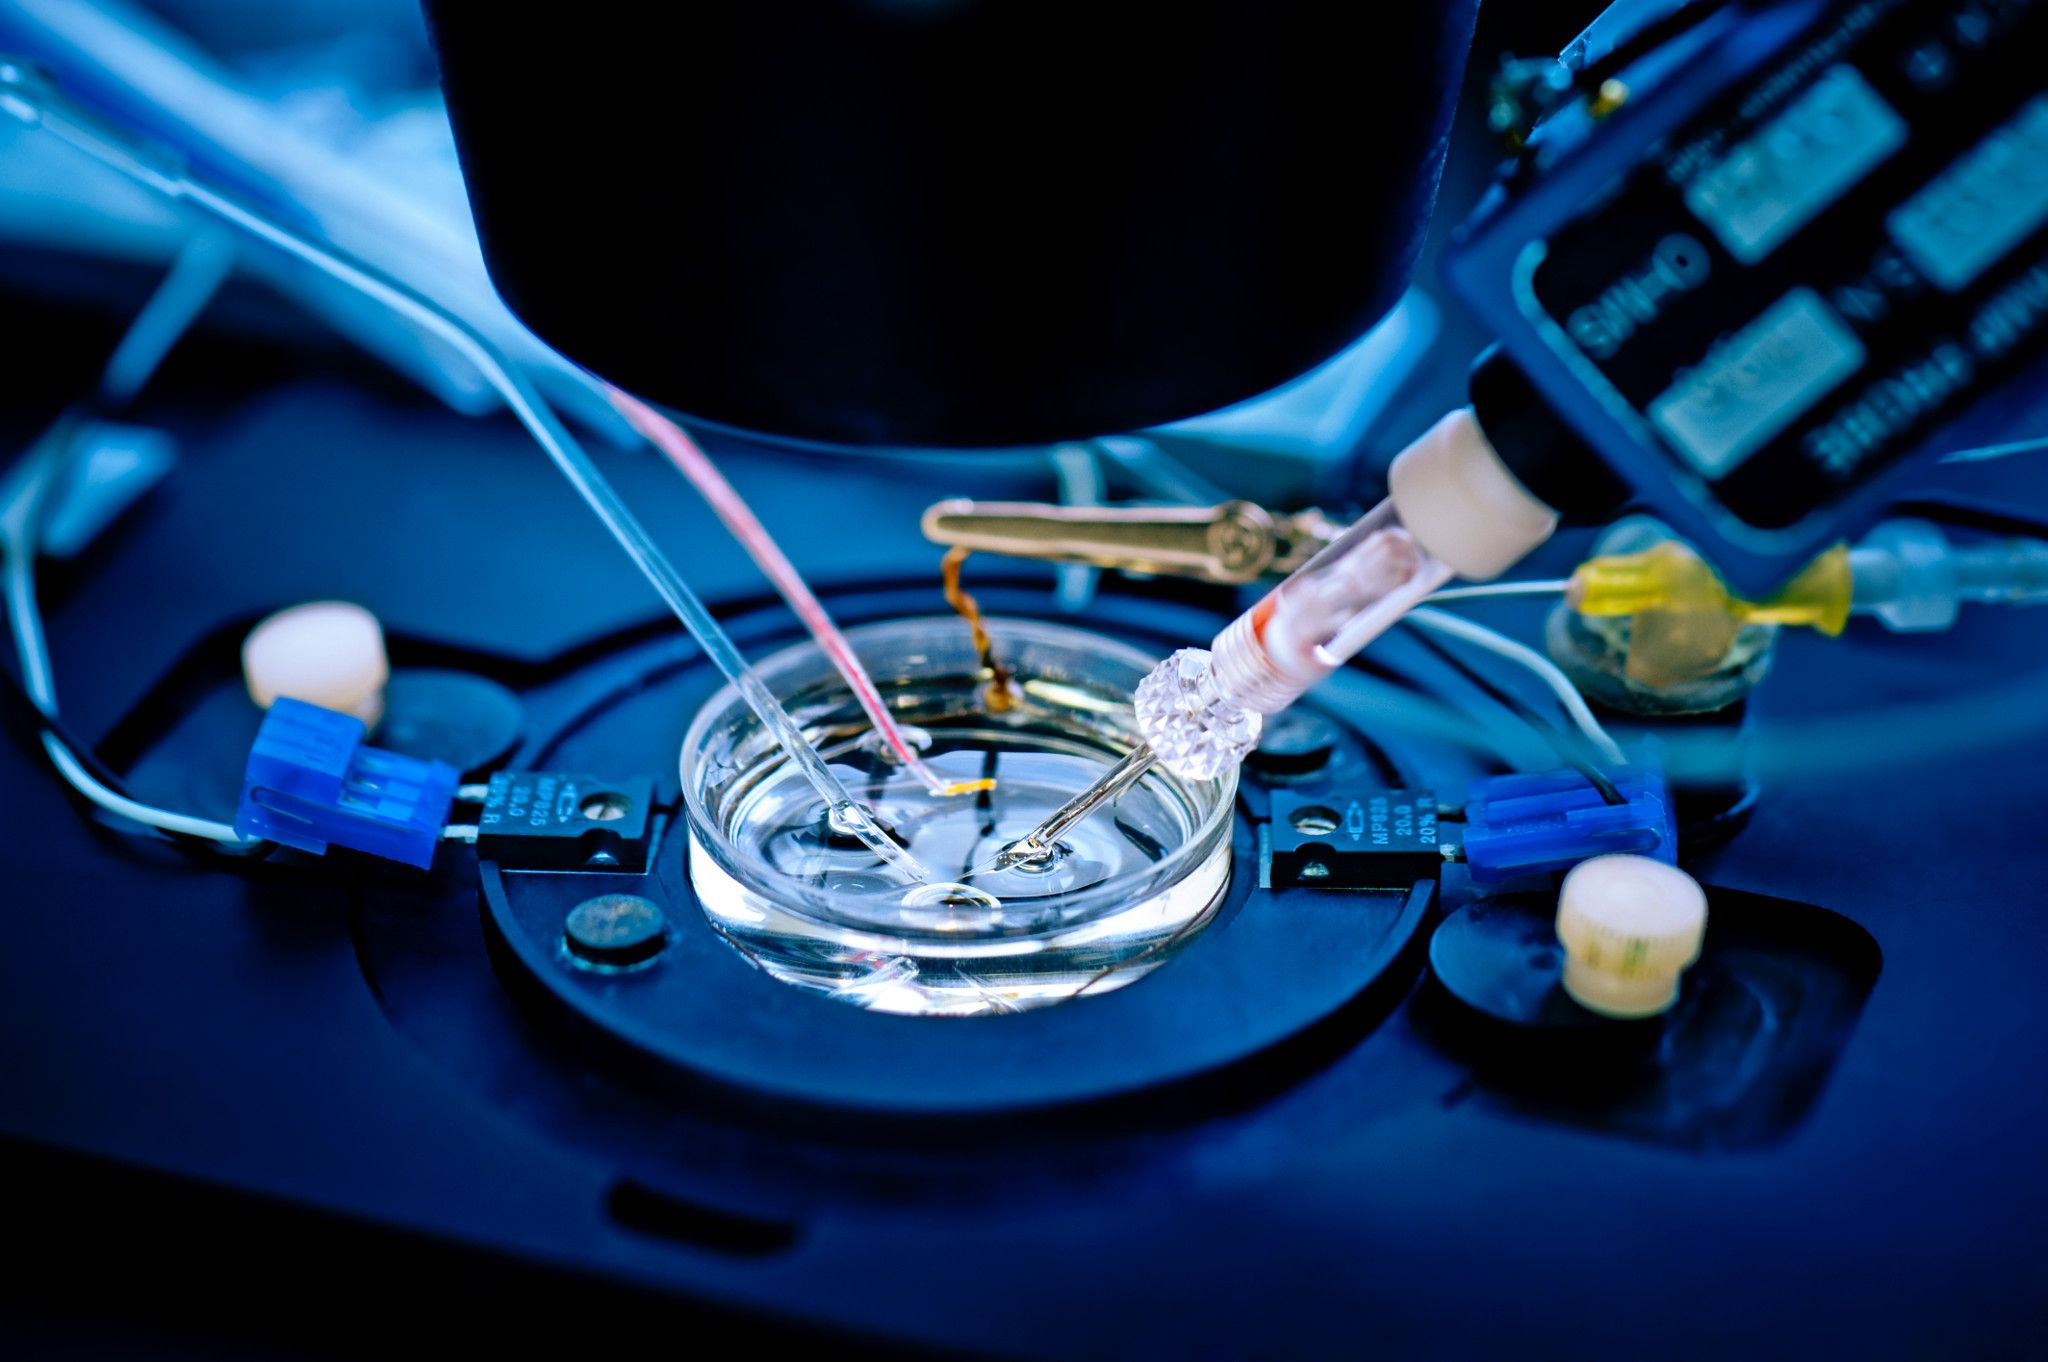
\includegraphics[width=\linewidth]{../../figures/patch-clamp-system.jpeg}
          \caption{Patch-Clamp System \cite{2025-patch-clamp-image}}
        \end{figure}
      \end{column}
      \begin{column}{0.58\linewidth}
        Approach in which electrophysiological behaviour of a cell can be measured in a lab.
        \begin{itemize}
          \item Cell-attached recording method
          \item Whole-cell recording method
        \end{itemize}
      \end{column}
    \end{columns}
  \end{frame}

  \begin{frame}{Simulation of the Experiment}
    %% Multiple independent Ion Channels
    %% Each follows: $$
  \end{frame}

  \begin{frame}{Hidden Markov Model}
    %% very nice, describe transition matrix and dependence on V, t
    The whole cell current $I: T \to \R$ over time $t \in T \subset \R^+$ is the sum of all individual channel contributions $I_k, k \in \{1, ..., M\}$ over $M \in \N$ channel types
    \begin{equation*}
      I(t) := \sum_{k=1}^{M} N_k I_k(t) = \sum_{k=1}^{M} N_k g_k p_{o,k} \left(V(t)-E_k\right)\,.
      \label{eq:current}
    \end{equation*}
    % where $N_k$ is the number of channels of type $k \in \{1, ..., M\}$, $g_k$ is the respective ion channel's conductivity, $p_{o, k} \in [0, 1]$ is the probability of observing the channel in a state where an ion current can flow (``open states''), $V: T \to \R$ is the voltage across the membrane and $E_k \in \R$ the reversal potential.

    At each time step, the next state $\vec{s}_{k,n+1} \in [0, 1]^{N_{s,k}}$ of the $k$-th channel type is obtained by
    \begin{equation*}
      \vec{s}_{k,n+1} = H_{k}\left(V(t_n), \vec{C}(t_n), t_n\right) \vec{s}_{k,n}\,,
      \quad\text{with}\quad
      t_n := \sum_{i=0}^n (\Delta t)_i\,.
    \end{equation*}
    % where $\vec{s}_{k,n} \in [0, 1]^{N_{s,k}}$ is the state vector of ion channel type $k$ at the $n$-th time step, $H_{k}\left(V, \vec{C}, t_n\right) \in [0, 1]^{N_{s,k} \times N_{s,k}}$ the transition matrix for type $k$ with $\sum_{j=1}^{N_{s,k}} \{H_k\}_{i,j} = 1 \;\forall\,i$, $V(t_n)$ the voltage across the membrane at time $t_n$ and $\vec{C}(t_n) \in \R^4$ the concentrations of Kalium, Calcium, Sodium and Chlorine at time $t_n$.
  \end{frame}

  \begin{frame}{Solution of the Inverse Problem}
    %% using different methods, based on LSQ.
    %% reformulation into a quadratic problem
  \end{frame}

  \begin{frame}{Runtime Optimisation}
    %% using adaptive timestepping

  \end{frame}

  \begin{frame}{Visualisation Dashboard}
    %% Based on Astro and @observablehq/plot, but mostly:

  \end{frame}
  \begin{frame}{WebAssembly}
    %% Compilation of Rust code
    %% Solver: [insert]
  \end{frame}

  \section{Simulation}
  \begin{frame}{Cancer Cell Simulation}
    \begin{itemize}
      \item Let's go!
    \end{itemize}
  \end{frame}

  \begin{frame}[allowframebreaks]{References}
    \printbibliography
  \end{frame}
\end{document}
